% Diagrammi di stato (sezione Behaviour del report).
% Sorgente TikZ autonomo come architettura.tex: ogni tikzpicture diventa una
% PAGINA del PDF, e il report sceglie il diagramma con \includegraphics[page=N].
%   cd doc/figures && latexmk -pdf diagrammi-stato.tex && latexmk -c diagrammi-stato.tex
% Pagine: 1 incidente, 2 change stream di un pod, 3 leader election, 4 sessione
% del client. Guardie, tempi e nomi degli eventi vanno tenuti allineati al
% codice (api/src/config.js, routes/, realtime/, tasks/, web/src/composables/).
\documentclass[tikz,border=3pt]{standalone}
\usepackage[T1]{fontenc}
\usepackage{lmodern}
\usetikzlibrary{arrows.meta,positioning,fit,calc,backgrounds}

\definecolor{edge}{HTML}{3B4252}
\definecolor{muted}{HTML}{5F6672}
\definecolor{stfill}{HTML}{EEF0FA}   \definecolor{stline}{HTML}{4B55A0}
\definecolor{okfill}{HTML}{EAF4F1}   \definecolor{okline}{HTML}{2F7564}
\definecolor{kofill}{HTML}{FBECEA}   \definecolor{koline}{HTML}{A3402F}
\definecolor{endfill}{HTML}{F1F1F1}  \definecolor{endline}{HTML}{5F6672}

\tikzset{
  font=\sffamily\scriptsize,
  >={Stealth[length=2mm,width=1.5mm]},
  state/.style={draw=#1line, fill=#1fill, rounded corners=5pt, line width=0.8pt,
                align=center, inner sep=4pt, minimum height=0.9cm, minimum width=2.3cm,
                font=\sffamily\footnotesize},
  state/.default=st,
  composite/.style={draw=#1line, fill=#1fill!45, rounded corners=7pt, line width=0.8pt,
                    inner sep=7pt},
  init/.style={circle, fill=edge, minimum size=6pt, inner sep=0pt},
  final/.style={circle, draw=edge, line width=0.8pt, minimum size=9pt, inner sep=0pt,
                path picture={\fill[edge] (path picture bounding box.center) circle (2.4pt);}},
  tr/.style={->, draw=edge, line width=0.7pt},
  lab/.style={font=\sffamily\scriptsize, text=edge, align=center, inner sep=1.5pt},
  note/.style={font=\sffamily\scriptsize\itshape, text=muted, align=left},
  ctitle/.style={font=\sffamily\footnotesize\bfseries, text=#1line},
}
% Etichetta di una transizione: evento [guardia] / azione.
\newcommand{\ev}[1]{\textbf{#1}}

\begin{document}

% =====================================================================
% 1. Ciclo di vita di un incidente (status su Mongo x claim su Redis)
% =====================================================================
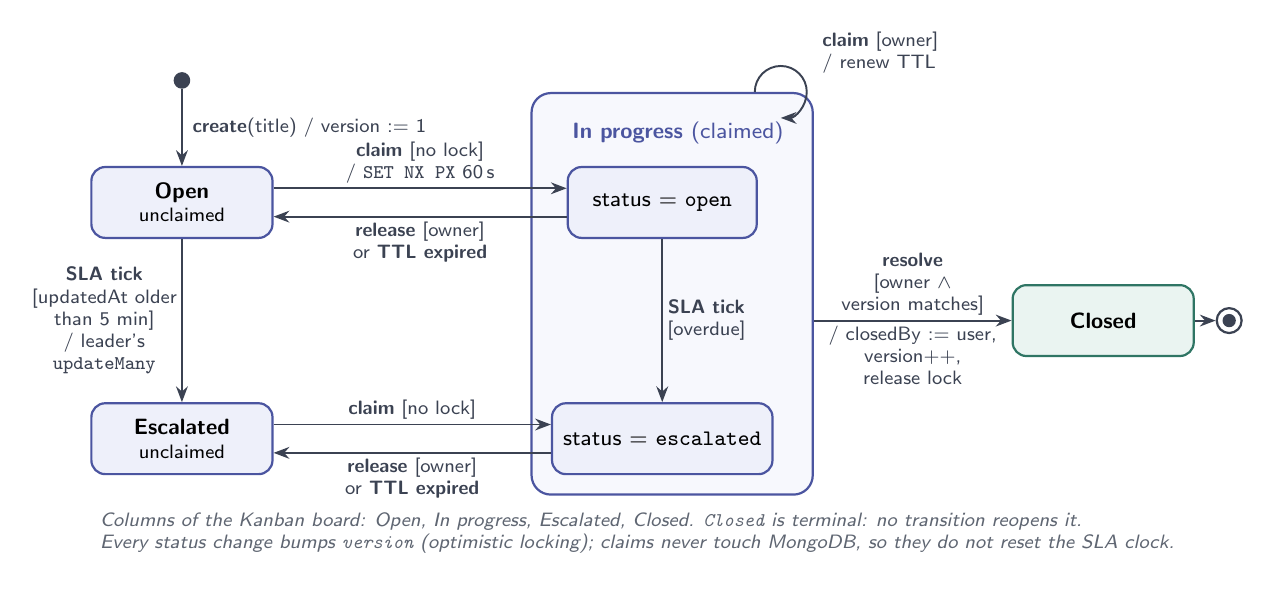
\begin{tikzpicture}
\node[init] (i) at (2.0,4.55) {};
\node[state] (open) at (2.0,3.0) {\textbf{Open}\\[-1pt]{\scriptsize unclaimed}};
\node[state] (esc)  at (2.0,0.0) {\textbf{Escalated}\\[-1pt]{\scriptsize unclaimed}};

\node[state, minimum width=2.4cm] (pOpen) at (8.1,3.0) {status = \texttt{open}};
\node[state, minimum width=2.4cm] (pEsc)  at (8.1,0.0) {status = \texttt{escalated}};
\node[ctitle=st, anchor=south west] (ptitle) at ($(pOpen.north west)+(-0.05,0.15)$) {In progress \textmd{(claimed)}};
\begin{scope}[on background layer]
  \node[composite=st, fit=(ptitle)(pOpen)(pEsc)] (prog) {};
\end{scope}

\node[state=ok] (closed) at (13.7,1.5) {\textbf{Closed}};
\node[final] (f) at (15.3,1.5) {};

\draw[tr] (i) -- node[lab, right=2pt] {\ev{create}(title) / version := 1} (open.north);

% Escalation SLA: anche sui ticket presi in carico.
\draw[tr] (open) -- node[lab, left] {\ev{SLA tick}\\{[}updatedAt older\\than 5 min{]}\\/ leader's\\\texttt{updateMany}} (esc);
\draw[tr] (pOpen) -- node[lab, right] {\ev{SLA tick}\\{[}overdue{]}} (pEsc);

% Presa in carico e rilascio, nei due stati di partenza.
\draw[tr] ($(open.east)+(0,0.18)$) -- node[lab, above] {\ev{claim} {[}no lock{]}\\/ \texttt{SET NX PX} 60\,s} ($(pOpen.west)+(0,0.18)$);
\draw[tr] ($(pOpen.west)+(0,-0.18)$) -- node[lab, below] {\ev{release} {[}owner{]}\\or \ev{TTL expired}} ($(open.east)+(0,-0.18)$);
\draw[tr] ($(esc.east)+(0,0.18)$) -- node[lab, above] {\ev{claim} {[}no lock{]}} ($(pEsc.west)+(0,0.18)$);
\draw[tr] ($(pEsc.west)+(0,-0.18)$) -- node[lab, below] {\ev{release} {[}owner{]}\\or \ev{TTL expired}} ($(esc.east)+(0,-0.18)$);

% Rinnovo idempotente del proprietario.
\draw[tr] ($(prog.north east)+(-0.75,0)$) arc[start angle=180, end angle=-90, radius=0.33];
\node[lab, anchor=west, align=left] at ($(prog.north east)+(0.05,0.5)$) {\ev{claim} {[}owner{]}\\/ renew TTL};

% Risoluzione: solo il proprietario, con la versione corrente.
\draw[tr] (prog.east |- closed) -- node[lab, above] {\ev{resolve}\\{[}owner $\wedge$\\version matches{]}} node[lab, below] {/ closedBy := user,\\version++,\\release lock} (closed);
\draw[tr] (closed) -- (f);

\node[note, anchor=north west] at ($(esc.south west)+(0,-0.35)$)
  {Columns of the Kanban board: \textit{Open}, \textit{In progress}, \textit{Escalated}, \textit{Closed}. \texttt{Closed} is terminal: no transition reopens it.\\
   Every status change bumps \texttt{version} (optimistic locking); claims never touch MongoDB, so they do not reset the SLA clock.};
\end{tikzpicture}

% =====================================================================
% 2. Change Stream di un pod api e readiness
% =====================================================================
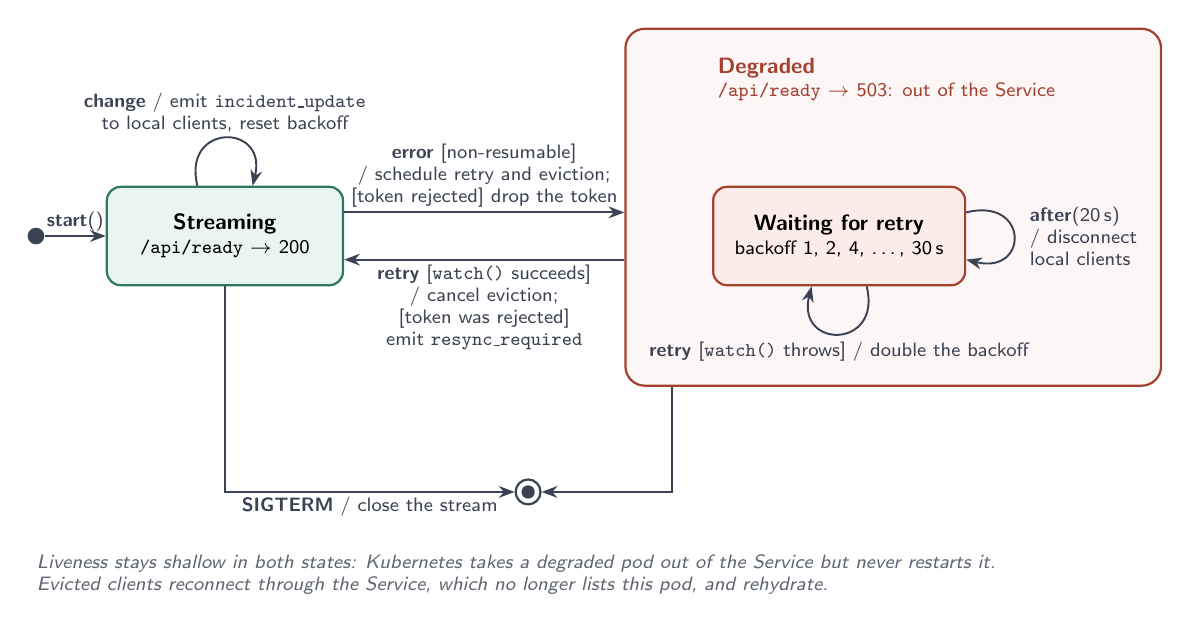
\begin{tikzpicture}
\node[init] (i) at (0,2.0) {};
\node[state=ok, minimum width=3.0cm, minimum height=1.25cm] (run) at (2.4,2.0)
  {\textbf{Streaming}\\[-1pt]{\scriptsize \texttt{/api/ready} $\to$ 200}};

\node[state=ko, minimum width=3.2cm, minimum height=1.25cm] (wait) at (10.2,2.0)
  {\textbf{Waiting for retry}\\[-1pt]{\scriptsize backoff 1, 2, 4, \ldots, 30\,s}};
\node[ctitle=ko, anchor=south west, align=left] (dtitle) at ($(wait.north west)+(-0.05,0.95)$)
  {Degraded\\[-1pt]\textmd{\scriptsize\texttt{/api/ready} $\to$ 503: out of the Service}};

% Ripianificazione: watch() fallisce in modo sincrono, nessuno stream nasce.
\draw[tr] ($(wait.south)+(0.35,0)$) .. controls +(0.2,-0.8) and +(-0.2,-0.8) .. ($(wait.south)+(-0.35,0)$);
\node[lab, anchor=north] (thr) at ($(wait.south)+(0,-0.65)$) {\ev{retry} {[}\texttt{watch()} throws{]} / double the backoff};
% Eviction dei client locali dopo 20 s di degrado.
\draw[tr] ($(wait.east)+(0,0.3)$) .. controls +(0.8,0.2) and +(0.8,-0.2) .. ($(wait.east)+(0,-0.3)$);
\node[lab, anchor=west, align=left] (evi) at ($(wait.east)+(0.75,0)$) {\ev{after}(20\,s)\\/ disconnect\\local clients};
\begin{scope}[on background layer]
  \node[composite=ko, fit=(dtitle)(wait)(thr)(evi)] (deg) {};
\end{scope}

\node[final] (f) at (6.25,-1.25) {};

\draw[tr] (i) -- node[lab, above] {\ev{start}()} (run);
\draw[tr] ($(run.north)+(-0.35,0)$) .. controls +(-0.2,0.8) and +(0.2,0.8) .. ($(run.north)+(0.35,0)$);
\node[lab, anchor=south] at ($(run.north)+(0,0.62)$) {\ev{change} / emit \texttt{incident\_update}\\to local clients, reset backoff};

\draw[tr] ($(run.east)+(0,0.3)$) -- node[lab, above] {\ev{error} {[}non-resumable{]}\\/ schedule retry and eviction;\\{[}token rejected{]} drop the token} ($(run.east -| deg.west)+(0,0.3)$);
\draw[tr] ($(run.east -| deg.west)+(0,-0.3)$) -- node[lab, below] {\ev{retry} {[}\texttt{watch()} succeeds{]}\\/ cancel eviction;\\{[}token was rejected{]}\\emit \texttt{resync\_required}} ($(run.east)+(0,-0.3)$);

\draw[tr] (run.south) |- node[lab, below, pos=0.75] {\ev{SIGTERM} / close the stream} (f);
\draw[tr] ($(deg.south west)+(0.6,0)$) |- (f);

\node[note, anchor=north west] at ($(i.west |- f.south)+(0,-0.5)$)
  {Liveness stays shallow in both states: Kubernetes takes a degraded pod out of the Service but never restarts it.\\
   Evicted clients reconnect through the Service, which no longer lists this pod, and rehydrate.};
\end{tikzpicture}

% =====================================================================
% 3. Leader election (per pod)
% =====================================================================
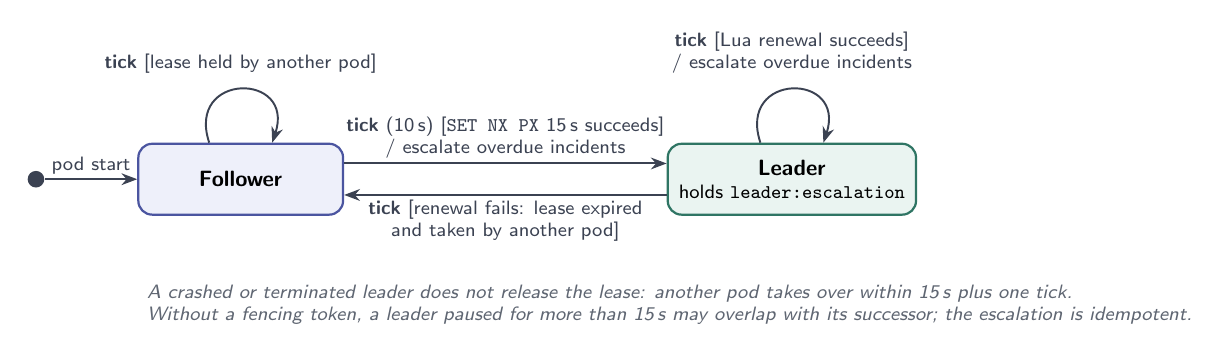
\begin{tikzpicture}
\node[init] (i) at (0,0) {};
\node[state, minimum width=2.6cm] (fol) at (2.6,0) {\textbf{Follower}};
\node[state=ok, minimum width=2.6cm] (lead) at (9.6,0) {\textbf{Leader}\\[-1pt]{\scriptsize holds \texttt{leader:escalation}}};

\draw[tr] (i) -- node[lab, above] {pod start} (fol);
\draw[tr] ($(fol.east)+(0,0.2)$) -- node[lab, above] {\ev{tick} (10\,s) {[}\texttt{SET NX PX} 15\,s succeeds{]}\\/ escalate overdue incidents} ($(lead.west)+(0,0.2)$);
\draw[tr] ($(lead.west)+(0,-0.2)$) -- node[lab, below] {\ev{tick} {[}renewal fails: lease expired\\and taken by another pod{]}} ($(fol.east)+(0,-0.2)$);

\draw[tr] ($(fol.north)+(-0.4,0)$) .. controls +(-0.3,0.9) and +(0.3,0.9) .. ($(fol.north)+(0.4,0)$)
  node[lab, above, pos=0.5, yshift=4pt] {\ev{tick} {[}lease held by another pod{]}};
\draw[tr] ($(lead.north)+(-0.4,0)$) .. controls +(-0.3,0.9) and +(0.3,0.9) .. ($(lead.north)+(0.4,0)$)
  node[lab, above, pos=0.5, yshift=4pt] {\ev{tick} {[}Lua renewal succeeds{]}\\/ escalate overdue incidents};

\node[note, anchor=north west] at ($(fol.south west)+(0,-0.75)$)
  {A crashed or terminated leader does not release the lease: another pod takes over within 15\,s plus one tick.\\
   Without a fencing token, a leader paused for more than 15\,s may overlap with its successor; the escalation is idempotent.};
\end{tikzpicture}

% =====================================================================
% 4. Sessione del client (browser)
% =====================================================================
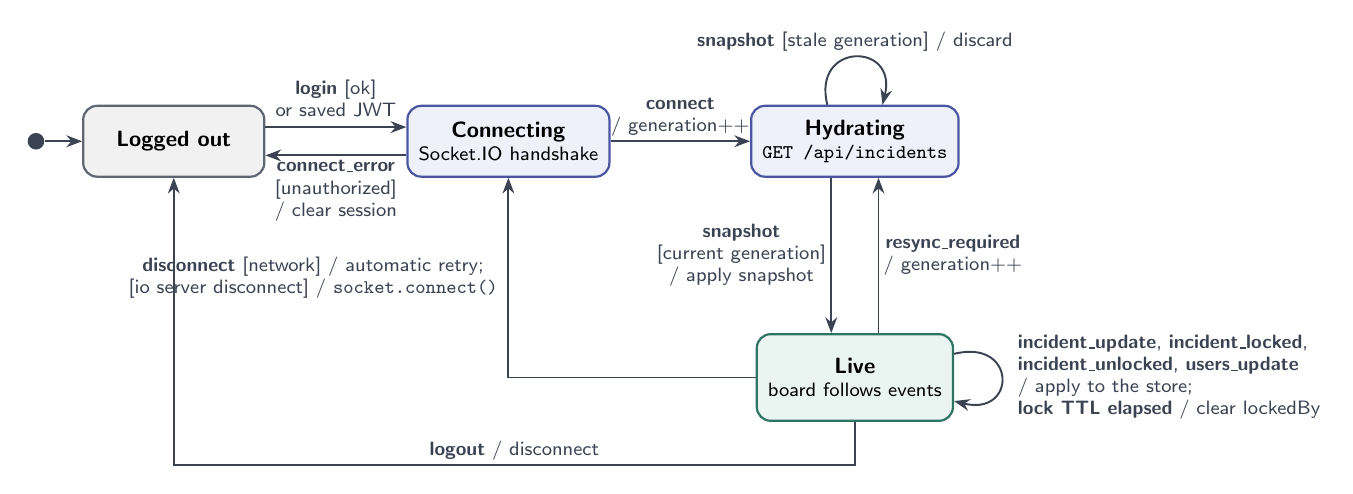
\begin{tikzpicture}
\node[init] (i) at (0,3.0) {};
\node[state=end, minimum width=2.3cm] (out) at (1.75,3.0) {\textbf{Logged out}};
\node[state, minimum width=2.4cm] (conn) at (6.0,3.0) {\textbf{Connecting}\\[-1pt]{\scriptsize Socket.IO handshake}};
\node[state, minimum width=2.4cm] (hyd) at (10.4,3.0) {\textbf{Hydrating}\\[-1pt]{\scriptsize \texttt{GET /api/incidents}}};
\node[state=ok, minimum width=2.4cm, minimum height=1.1cm] (live) at (10.4,0.0) {\textbf{Live}\\[-1pt]{\scriptsize board follows events}};

\draw[tr] (i) -- (out);
\draw[tr] ($(out.east)+(0,0.18)$) -- node[lab, above=2pt] {\ev{login} {[}ok{]}\\or saved JWT} ($(conn.west)+(0,0.18)$);
\draw[tr] ($(conn.west)+(0,-0.18)$) -- node[lab, below] {\ev{connect\_error}\\{[}unauthorized{]}\\/ clear session} ($(out.east)+(0,-0.18)$);
\draw[tr] (conn) -- node[lab, above] {\ev{connect}\\/ generation++} (hyd);

\draw[tr] ($(hyd.south)+(-0.3,0)$) -- node[lab, left] {\ev{snapshot}\\{[}current generation{]}\\/ apply snapshot} ($(live.north)+(-0.3,0)$);
\draw[tr] ($(live.north)+(0.3,0)$) -- node[lab, right] {\ev{resync\_required}\\/ generation++} ($(hyd.south)+(0.3,0)$);

\draw[tr] ($(hyd.north)+(-0.35,0)$) .. controls +(-0.2,0.8) and +(0.2,0.8) .. ($(hyd.north)+(0.35,0)$);
\node[lab, anchor=south] at ($(hyd.north)+(0,0.62)$) {\ev{snapshot} {[}stale generation{]} / discard};

\draw[tr] ($(live.east)+(0,0.3)$) .. controls +(0.8,0.2) and +(0.8,-0.2) .. ($(live.east)+(0,-0.3)$);
\node[lab, anchor=west, align=left] at ($(live.east)+(0.75,0)$)
  {\ev{incident\_update}, \ev{incident\_locked},\\\ev{incident\_unlocked}, \ev{users\_update}\\/ apply to the store;\\\ev{lock TTL elapsed} / clear lockedBy};

\draw[tr] (live.west) -| node[lab, left=2pt, pos=0.75] {\ev{disconnect} {[}network{]} / automatic retry;\\{[}io server disconnect{]} / \texttt{socket.connect()}} (conn.south);
\draw[tr] (live.south) -- ++(0,-0.55) -| node[lab, above, pos=0.25] {\ev{logout} / disconnect} (out.south);
\end{tikzpicture}

\end{document}
